\subsection{Roulette Selection}
El mecanismo de selección de ruleta, es una técnica popularmente usada en algoritmos genéticos para seleccionar posibles soluciones de acuerdo a su aptitud. La idea es dar a cada individuo una probabilidad de ser seleccionado que sea proporcional a su aptitud, de tal manera que los individuos con mayor aptitud tengan una mayor probabilidad de ser elegidos, pero aún permitiendo que los individuos con menor aptitud tengan alguna posibilidad.

En términos generales, este método consta de los siguientes pasos:

\begin{enumerate}
	\item Cálculo de Aptitudes: En primer lugar, se calcula la aptitud de cada individuo en la población.
	\item Suma de Aptitudes: Se suman todas las aptitudes para obtener una aptitud total de la población.
	\item Cálculo de Probabilidades: Se determina la probabilidad de selección de cada individuo dividiendo su aptitud por la aptitud total de la población.
	\item Selección: Se genera un número aleatorio entre 0 y 1. Luego, se selecciona el individuo cuya probabilidad acumulada incluye este número aleatorio. En otras palabras, imaginamos que giramos una ruleta donde cada segmento corresponde a un individuo, y el tamaño de cada segmento es proporcional a la aptitud del individuo.
\end{enumerate}

Una representación gráfica de este mecanismo se puede observar en la Figura \ref{fig:RS}.

\begin{figure}[htbp]
	\centering
	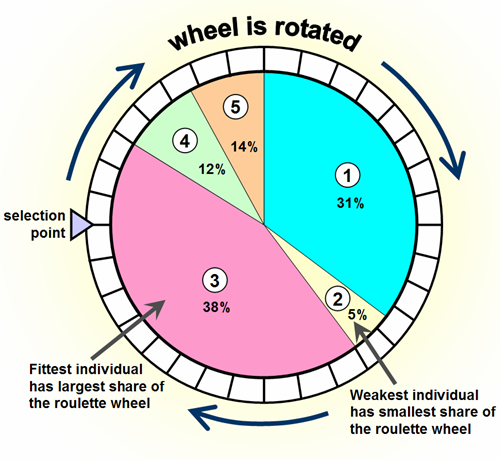
\includegraphics[width=0.4\textwidth]{roulette_selection}
	\caption{Diagrama de funcionamiento de selección por ruleta.}
	\label{fig:RS}
\end{figure}


\subsection{Two Point Crossover}
La cruza de dos puntos (two point crossover, en inglés) es un método de recombinación comúnmente utilizado en algoritmos genéticos que permite la combinación de características de dos padres para generar una descendencia. Este método permite generar combinaciones de características de ambos padres para explorar y buscar mejores soluciones. En terminos generales, este método consta de los siguientes pasos:

\begin{enumerate}
	\item Definición de Puntos de Corte: Se seleccionan dos puntos de corte en la representación de los padres. Estos puntos dividen a los padres en tres segmentos: el segmento antes del primer punto de corte, el segmento entre los dos puntos de corte y el segmento después del segundo punto de corte.
	\item Creación de Descendencia: La descendencia se crea intercambiando los segmentos intermedios (el segmento entre los dos puntos de corte) de los dos padres. El resultado es un nuevo individuo que combina partes de ambos padres.
\end{enumerate}

\begin{figure}[htbp]
	\centering
	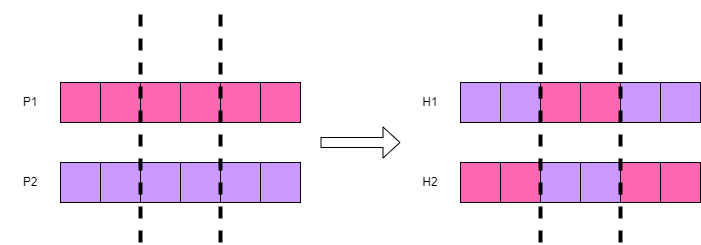
\includegraphics[width=0.8\textwidth]{crossover_two}
	\caption{Mecanismo de cruza de dos puntos.}
	\label{fig: cross_two}
\end{figure}


\subsection{Scramble Mutation}
La mutación por mezcla (scramble mutation, en inglés) es un proceso que introduce pequeños cambios aleatorios en los individuos de una población con el objetivo de aumentar la diversidad genética y explorar nuevas soluciones en el espacio de búsqueda. Dicho proceso se caracteriza por los siguientes pasos:

\begin{enumerate}
	\item Selección de un subconjunto de genes: Se elige un subconjunto aleatorio de genes en la representación del individuo. Los genes seleccionados formarán parte del proceso de mutación.
	\item Mezcla de genes: Los genes seleccionados se reordenan de manera aleatoria entre sí. Este reordenamiento aleatorio puede ser realizado de diferentes maneras, como permutando los valores de los genes dentro del subconjunto o cambiando su posición en la secuencia.
\end{enumerate}

Podemos observar una representación gráfica de este mecanismo en la Figura \ref{fig:scrM}.

\begin{figure}[htbp]
	\centering
	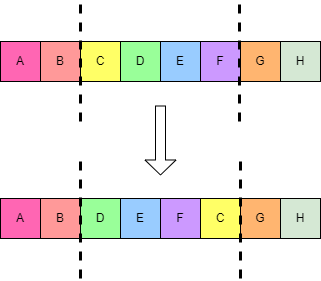
\includegraphics[width=0.4\textwidth]{scramble_mutation}
	\caption{Diagrama de funcionamiento de scramble mutation.}
	\label{fig:scrM}
\end{figure}


\subsection{Competencia genética}
El concepto de competencia genética se asemeja a la lucha por la supervivencia en la naturaleza, donde los individuos más aptos tienen una mayor probabilidad de sobrevivir y reproducirse, transmitiendo así sus genes a la siguiente generación. La idea principal detrás de la competencia genética en algoritmos evolutivos es simular este proceso de selección natural para buscar soluciones óptimas o mejores en un espacio de búsqueda.

En este proceso se toma a todos los padres y a todos los hijos, se ordenan de mayor a menor aptitud, y solamente se permitirá que pasen a la siguiente generación aquellos que presentan mejor aptitud, sin importar sin son padres o hijos.
